\section{幂零元与既约环}\label{sec:nilpotents-and-reduced-rings}

由 Corollary~\ref{cor:coordinate-ring-finitely-generated} 可知, 仿射簇 $X$ 的坐标环 $K[X]$ 是一个有限生成的 $K$-代数. 这一点来自对 $K[X]$ 的商环解释:
\[
  K[X]=K[x_{1},\ldots,x_{n}]/\mathcal{I}(X).
\]
不过, 这个商环还有一个重要方面没有考虑: $K[X]$ 不是对任意理想取商, 而是对根理想取商. 那么, $\mathcal{I}(X)$ 是根理想这一事实, 对坐标环 $K[X]$ 的代数性质意味着什么? 这个问题的答案可以用以下定义表述.

\begin{Definition}{幂零元与既约环}\leavevmode\label{def:nilpotent-elements-and-reduced-rings}
  设 $R$ 是一个环. 若存在整数 $m\geq1$ 使得 $a^{m}=0$, 则称元素 $a\in R$ 是\textbf{幂零的}. 如果 $R$ 没有非零幂零元, 就称 $R$ 是\textbf{既约的}.
\end{Definition}

\begin{Example}{既约环}\leavevmode\label{ex:reduced-ring-not-domain}
  任何整环都必定是既约的, 因为非零幂零元会是零因子. 不过, 并非所有既约环都是整环. 例如, 商环
  \[
    \frac{K[x,y]}{\langle xy\rangle}
  \]
  不是整环, 因为 $[x]$ 和 $[y]$ 是零因子, 但它是既约的. 要说明这个环是既约的, 假设 $[f]^{m}=0$, 必须证明 $[f]=0$. 因为
  \[
    [f^{m}]=[f]^{m}=0\in\frac{K[x,y]}{\langle xy\rangle},
  \]
  可知 $xy$ 整除 $f^{m}$, 这蕴含 $x$ 和 $y$ 都整除 $f^{m}$. 由于 $x$ 和 $y$ 在 $K[x,y]$ 中不可约, 因而是素元, 可得 $x$ 和 $y$ 都整除 $f$. 所以 $xy$ 整除 $f$, 且 $[f]=0$. 因而该环不含任何非零幂零元, 所以它是既约的.
\end{Example}

整环都是既约环而反之不然, 正反映出素理想都是根理想而反之不然 (见 Proposition~\ref{prop:quotient-reduced-iff-ideal-radical}).

\begin{Example}{一个非既约环}\leavevmode\label{ex:nonreduced-ring}
  商环
  \[
    \frac{K[x]}{\langle x^{2}\rangle}
  \]
  不是既约的, 因为它有非零幂零元:
  \[
    [x]\ne0\qquad\text{满足}\qquad[x]^{2}=0.
  \]
\end{Example}

下面的结果用商环刻画根理想, 类似于用商环刻画素理想与极大理想的结果.

\begin{Proposition}{对根理想取商}\leavevmode\label{prop:quotient-reduced-iff-ideal-radical}
  理想 $I\subseteq R$ 是根理想, 当且仅当 $R/I$ 是既约的.
\end{Proposition}

\begin{Proof}
  见 Exercise~\ref{ex:prove-quotient-reduced-iff-ideal-radical}.
\end{Proof}

现在可以从代数上完整刻画哪些环可以作为 $K$ 上的仿射簇的坐标环: 它们是作为环既约的有限生成 $K$-代数.

\begin{Proposition}{坐标环的刻画}\leavevmode\label{prop:coordinate-rings-as-finitely-generated-reduced-algebras}
  若 $X\subseteq\mathbb{A}^{n}$ 是一个仿射簇, 则坐标环 $K[X]$ 是有限生成的既约 $K$-代数. 反过来, 若 $A$ 是有限生成的既约 $K$-代数, 则对某个仿射簇 $X\subseteq\mathbb{A}^{n}$, 有 $A\cong K[X]$.
\end{Proposition}

\begin{Proof}
  假设 $X$ 为仿射簇. 由 Proposition~\ref{prop:coordinate-ring-as-quotient-k-algebra},
  \[
    K[X]=K[x_{1},\ldots,x_{n}]/\mathcal{I}(X).
  \]
  因此, 由 Proposition~\ref{prop:characterization-of-finitely-generated-k-algebras} 可知 $K[X]$ 是有限生成的. 又因为 $\mathcal{I}(X)$ 是根理想, 由 Proposition~\ref{prop:quotient-reduced-iff-ideal-radical} 可知它是既约的.

  反过来, 假设 $A$ 是有限生成的既约 $K$-代数. 根据 Proposition~\ref{prop:characterization-of-finitely-generated-k-algebras}, 对某个 $n$ 和某个 $I$ 可以写成
  \[
    A\cong K[x_{1},\ldots,x_{n}]/I
  \]
  并且根据 Proposition~\ref{prop:quotient-reduced-iff-ideal-radical} 可知 $I$ 是根理想. 定义 $X=\mathcal{V}(I)\subseteq\mathbb{A}^{n}$. 由零点定理,
  \[
    \mathcal{I}(X)=\mathcal{I}(\mathcal{V}(I))=\sqrt{I}=I.
  \]
  再由 Proposition~\ref{prop:coordinate-ring-as-quotient-k-algebra} 可得 $A\cong K[X]$.
\end{Proof}

为了实际运用 Proposition~\ref{prop:coordinate-rings-as-finitely-generated-reduced-algebras}, 应当能在给定有限生成的既约 $K$-代数 $A$ 时, 找到一个满足 $K[X]\cong A$ 的仿射簇 $X$. 下例说明具体怎样做.

\begin{Example}{{由 \textmd{$K[X]$} 确定 $X$}}\leavevmode\label{ex:coordinate-ring-of-quadratic-subalgebra}
  设 $A$ 为子代数
  \[
    A=K[u^{2},uv,v^{2}]\subseteq K[u,v].
  \]
  那么 $A$ 显然是有限生成的, 因为它由 $u^{2}$, $uv$ 和 $v^{2}$ 这三个元素生成. 它也是既约的, 因为它是既约 $K$-代数 $K[u,v]$ 的子代数. 因此应当存在一个仿射簇 $X$, 使得 $K[X]\cong A$.

  为求出 $X$, 先给三个生成元取一些有提示作用的名字:
  \[
    x=u^{2},\quad y=uv,\quad\text{以及}\quad z=v^{2}.
  \]
  注意, 这三个生成元满足关系
  \[
    xz-y^{2}=(u^{2})(v^{2})-(uv)^{2}=0.
  \]
  考虑由此关系定义的仿射簇:
  \[
    X=\mathcal{V}(xz-y^{2})\subseteq\mathbb{A}^{3}.
  \]
  本例余下的部分证明 $K[X]\cong A$.

  首先注意多项式 $xz-y^{2}$ 不可约 (例如可用 Eisenstein 判别法), 所以理想 $\langle xz-y^{2}\rangle$ 是素理想, 因而是根理想. 由零点定理可得
  \[
    \mathcal{I}(X)=\mathcal{I}(\mathcal{V}(xz-y^{2}))
      =\sqrt{\langle xz-y^{2}\rangle}=\langle xz-y^{2}\rangle,
  \]
  所以
  \[
    K[X]\cong\frac{K[x,y,z]}{\langle xz-y^{2}\rangle}.
  \]
  剩下要证明的是
  \begin{equation}\label{eq:quadratic-subalgebra-presentation}
    \frac{K[x,y,z]}{\langle xz-y^{2}\rangle}\cong A.
  \end{equation}
  为证明 \eqref{eq:quadratic-subalgebra-presentation}, 定义 $K$-代数同态 $\phi:K[x,y,z]\to A$ 为
  \[
    \phi(f)=f(u^{2},uv,v^{2}).
  \]
  由于 $A$ 的三个生成元 $u^{2},uv,v^{2}$ 都在 $\phi$ 的像中, $\phi$ 是满射. 因此, 只要能证明 $\ker(\phi)=\langle xz-y^{2}\rangle$, 所求的同构 \eqref{eq:quadratic-subalgebra-presentation} 就可由 $K$-代数的第一同构定理得出.

  由于
  \[
    \phi(xz-y^{2})=(u^{2})(v^{2})-(uv)^{2}=0,
  \]
  $\langle xz-y^{2}\rangle$ 的每个元素都被 $\phi$ 映到 $0$, 所以 $\ker(\phi)\supseteq\langle xz-y^{2}\rangle$. 要证明反向的包含关系, 假设 $f\in\ker(\phi)$, 并考虑陪集
  \[
    [f]\in\frac{K[x,y,z]}{\langle xz-y^{2}\rangle}.
  \]
  反复利用等式 $[y^{2}]=[xz]$, 可知
  \[
    [f]=[g(x,z)+yh(x,z)]
  \]
  对某些多项式 $g,h\in K[x,z]$ 成立. 换句话说,
  \[
    f=g(x,z)+y\cdot h(x,z)+\ell(x,y,z)(xz-y^{2})
  \]
  对某个多项式 $\ell\in K[x,y,z]$ 成立. 对此式应用 $\phi$, 得到
  \[
    0=\phi(f)=g(u^{2},v^{2})+uv\cdot h(u^{2},v^{2})\in K[u,v].
  \]
  因为 $g(u^{2},v^{2})$ 这一项是 $u$ 和 $v$ 都只出现偶次幂的多项式, 而 $uv\cdot h(u^{2},v^{2})$ 这一项是 $u$ 和 $v$ 都只出现奇次幂的多项式, 这两项不能相消. 因此必有 $g=h=0$, 从而 $f\in\langle xz-y^{2}\rangle$. 于是 $\ker(\phi)\subseteq\langle xz-y^{2}\rangle$, 论证完毕.
\end{Example}

\hyperref[fig:coordinate-rings-venn-diagram]{下图}概括了本章的进展. 特别地, 在环的范畴中, 我们已经准确确定了哪些环可以作为 $K$ 上仿射簇的坐标环: 它们是既有限生成又既约的 $K$-代数.

\par\smallskip
{\centering
\begin{tikzpicture}
  \phantomsection\label{fig:coordinate-rings-venn-diagram}
  \node[inner sep=0pt,anchor=south west] (venn) at (0,0)
    {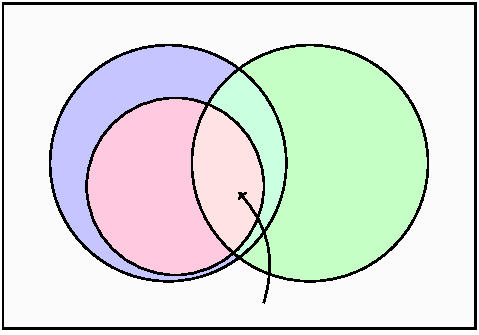
\includegraphics[width=.70\linewidth]{figures/coordinate-ring-venn-geometry.pdf}};
  \begin{scope}[x={(venn.south east)},y={(venn.north west)},every node/.style={font=\small,inner sep=0pt,align=center}]
    \node at (.50,.922) {环};
    \node at (.334,.762) {$K$-代数};
    \node at (.683,.740) {既约环};
    \node at (.327,.390) {有限生成的\\$K$-代数};
    \node at (.551,.061) {坐标环};
  \end{scope}
\end{tikzpicture}\par}
\smallskip

现在我们有了一套代数语言, 可以用来刻画和讨论坐标环. 下一章的目标是研究坐标环 $K[X]$ 能告诉我们有关仿射簇 $X$ 的哪些信息. 正如我们将看到的, 坐标环本质上知道与其对应的仿射簇的一切. 这一有力的事实使我们能够把环和 $K$-代数的所有代数工具用到仿射簇的研究中.

\BookExerciseHeading
\begin{BookExercises}
  \item\label{ex:subring-of-reduced-ring-is-reduced} 说明为什么既约环的任意子环都是既约的.
  \item\label{ex:prove-quotient-reduced-iff-ideal-radical} 证明 Proposition~\ref{prop:quotient-reduced-iff-ideal-radical}.
  \item\label{ex:direct-sums-and-reducedness}
    \begin{enumerate}[label=(\alph*)]
      \item 证明如果 $R$ 或 $S$ 是既约的, 则直和 $R\oplus S$ 是既约的. (回顾一下, 直和中的加法和乘法按分量定义.)
      \item 证明 $K$-代数 $A=K[x]/\langle x^{2}\rangle$ 与 $K\oplus K$ 作为 $K$-向量空间同构, 但作为环不同构.
    \end{enumerate}
  \item\label{ex:polynomial-rings-over-reduced-rings} 设 $R$ 是既约环. 证明 $R[x]$ 是既约的, 并用归纳法得出对任意 $n$, $R[x_{1},\ldots,x_{n}]$ 都是既约的.
  \item\label{ex:find-variety-of-subalgebra-square-cube} 设 $A=K[u^{2},u^{3}]\subseteq K[u]$.
    \begin{enumerate}[label=(\alph*)]
      \item 说明怎样知道 $A$ 是有限生成且既约的.
      \item 找出一个仿射簇 $X$, 使 $K[X]\cong A$, 并证明你的答案.
    \end{enumerate}
  \item\label{ex:find-affine-variety-of-linear-generators} 设 $A=K[u+w,v+w]\subseteq K[u,v,w]$. 找出一个仿射簇 $X$, 使 $K[X]\cong A$, 并证明你的答案.
  \item\label{ex:find-affine-variety-from-multiplication-table} 设 $A$ 是以
    \[
      \{x^{i}\mid i\geq0\}\cup\{x^{i}y\mid i\geq0\}
    \]
    为基的 $K$-向量空间. 在这些基元素上定义一个 (交换的) 乘积, 令
    \[
      \begin{aligned}
        x^{i}\cdot x^{j}&=x^{i+j},\\
        x^{i}\cdot x^{j}y&=x^{i+j}y,\qquad\text{并且}\\
        x^{i}y\cdot x^{j}y&=x^{i+j+3},
      \end{aligned}
    \]
    再以 $K$-线性的方式把这个乘积扩张到 $A$ 的所有元素.
    \begin{enumerate}[label=(\alph*)]
      \item 证明 $A$ 是有限生成的既约 $K$-代数.
      \item 找出一个仿射簇 $X$, 使 $K[X]\cong A$, 并证明你的答案.
    \end{enumerate}
  \item\label{ex:coordinate-ring-from-ideal-of-relations} 设 $a_{1},\ldots,a_{m}\in K[x_{1},\ldots,x_{n}]$, 考虑子代数
    \[
      A=K[a_{1},\ldots,a_{m}]\subseteq K[x_{1},\ldots,x_{n}].
    \]
    设 $I\subseteq K[y_{1},\ldots,y_{m}]$ 是 $a_{1},\ldots,a_{m}$ 的关系理想:
    \[
      f\in I\quad\Longleftrightarrow\quad
        f(a_{1},\ldots,a_{m})=0\in K[x_{1},\ldots,x_{n}].
    \]
    定义 $X=\mathcal{V}(I)\subseteq\mathbb{A}^{m}$. 证明 $K[X]\cong A$.
  \item\label{ex:examples-for-coordinate-ring-venn-regions} 对本节末尾\hyperref[fig:coordinate-rings-venn-diagram]{Venn 图}的每个区域, 各举一个属于该区域的环的明确例子.
\end{BookExercises}

\par\smallskip
{\footnotesize
\noindent\textbf{开放获取.} 本章按照
\href{http://creativecommons.org/licenses/by-nc/4.0/}{Creative Commons Attribution-NonCommercial 4.0 International License}
的条款授权. 该许可允许以任何媒介或格式进行非商业性使用, 分享, 改编, 分发和复制, 但须对原作者和来源作适当署名, 提供 Creative Commons 许可的链接, 并说明是否作了修改.

\noindent
\begin{minipage}[t]{.17\linewidth}
  \vspace{0pt}
\includegraphics[width=.9\linewidth]{figures/source-cc-by-nc.png}
\end{minipage}\hfill
\begin{minipage}[t]{.81\linewidth}
  \vspace{0pt}本章的图片或其他第三方材料均纳入本章的 Creative Commons 许可, 除非材料的署名行另有注明. 如果材料未纳入本章的 Creative Commons 许可, 且您拟进行的使用未获法律规定的许可或超出允许使用的范围, 则须直接向著作权持有人取得许可.
\end{minipage}\par}
